\section{系统设计与研究方法}

\subsection{总体流程}

系统以一次需求方向对应一个独立批次。批次首先保存需求描述、关键词、时间窗和来源请求记录；采集结果随后进行来源链接规范化、内容清理、相关性筛选和重复识别。清洗记录以批次号和连续编号关联正文快照。机会判别覆盖清洗结果中的全部记录，机会记录才进入语义表示、主题聚合和价值评估。决策支持层提供来源追溯、主题成员查询和策划案所需的证据接口。

图~\ref{fig:pipeline} 给出 B01 各处理阶段的数量变化。最后一列表示进入主题计算的人工确认机会候选，不能解释为已验证的市场机会。

\begin{table}[H]
  \centering
  \small
  \caption{赛题任务与系统处理结果}
  \label{tab:tasks}
  \begin{tabular}{@{}>{\raggedright\arraybackslash}p{0.16\textwidth}>{\raggedright\arraybackslash}p{0.39\textwidth}>{\raggedright\arraybackslash}p{0.35\textwidth}@{}}
    \toprule
    任务 & B01 结果 & 证据边界 \\
    \midrule
    采集清洗 & 共 2561 条清洗记录 & 公开检索样本 \\
    机会判别 & 共 2561 条全量人工确认标签，100 条机会 & 509 条逐条审阅标签，其余按授权登记 \\
    主题聚合 & 共 14 个人工确认主题 & 12 个单记录主题 \\
    价值排序 & 最高分为 C2（85.76） & 仅供探索筛选 \\
    决策支持 & 复核工作台、主题优先级视图与 C2 策划案 & 浏览器截图仍需补齐 \\
    \bottomrule
  \end{tabular}
\end{table}

\begin{figure}[H]
  \centering
  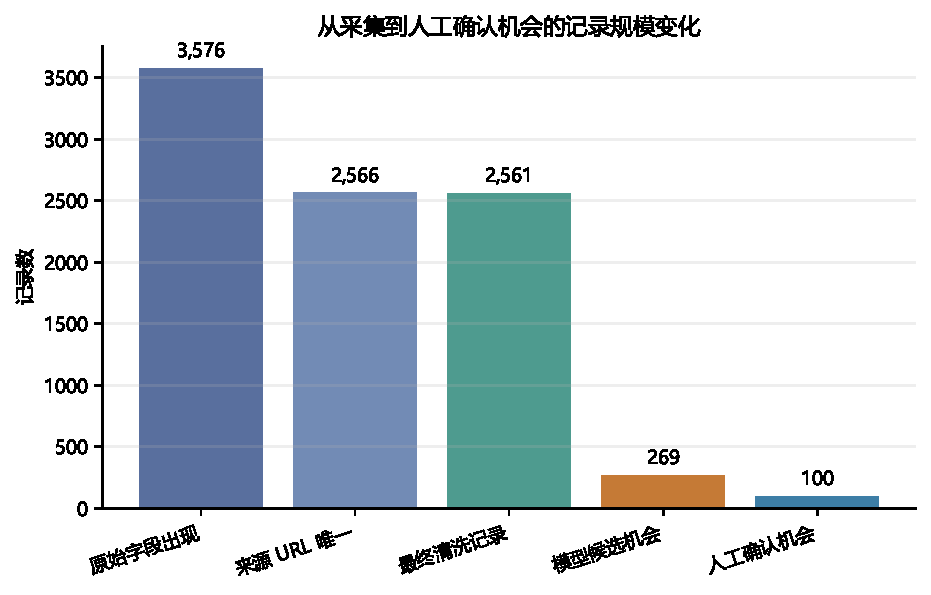
\includegraphics[width=0.92\textwidth]{../figures/fig02_pipeline_counts.pdf}
  \caption{B01 从采集到人工确认机会候选的记录规模。该图展示处理阶段计数，不表示采集召回率或分类准确率。}
  \label{fig:pipeline}
\end{figure}

为检查小样本条件下的神经网络分类是否改善机会标签复现，本文在人工确认样本上追加折外模型比较。该实验沿用结构化机会条件和分层复核边界，不改变全量自动判别结果。研究流程和证据关系如图~\ref{fig:method} 所示。

\begin{figure}[H]
  \centering
  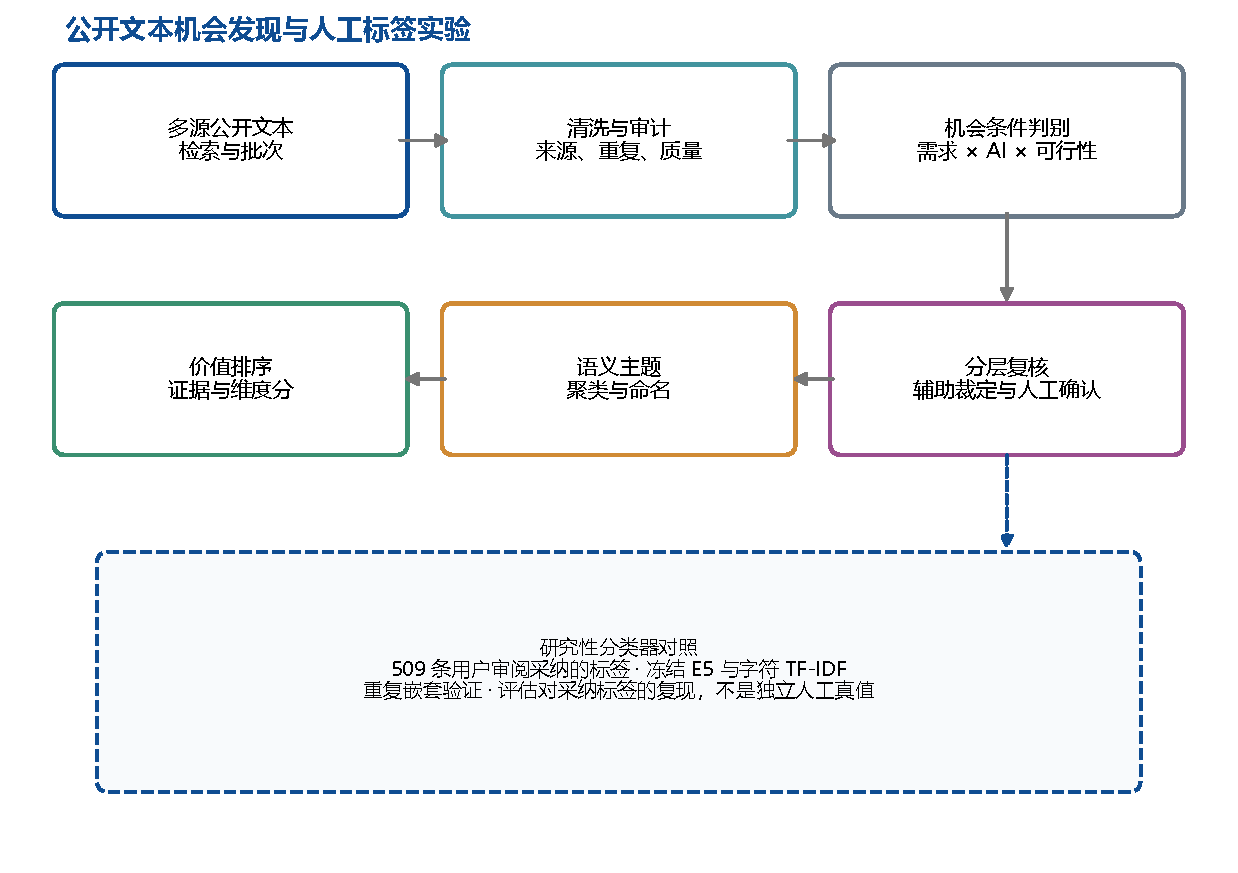
\includegraphics[width=0.98\textwidth]{../figures/fig15_opportunity_method.pdf}
  \caption{B01 机会发现流程与人工标签分类实验。下方模型比较评价对 509 条人工确认标签的复现能力。}
  \label{fig:method}
\end{figure}

\subsection{机会判别条件}

对记录 $i$ 定义四个布尔条件：$d_i$ 表示是否存在可观察的终端需求，$a_i$ 表示 AI 是否为解决路径的核心能力，$f_i$ 表示现有模型或成熟算法能否实现，$e_i$ 表示是否命中教程、科普、新闻、广告、融资宣传、开发者内部记录或测试任务等排除项。自动机会标签定义为

\begin{equation}
 y_i=d_i\land a_i\land f_i\land\neg e_i .
 \label{eq:opportunity}
\end{equation}

模型同时输出功能类别、行业类别、置信度、需求说明和正文证据。程序约束机会记录的功能和行业必须来自官方标签集合，并检查每条证据能在清洗后的正文中找到。非机会记录的两个分类字段保持为空。

\subsection{语义表示、聚类与价值评估}

主题聚合使用多语言文本向量表示标题和正文，采用 HDBSCAN 密度聚类。HDBSCAN 能在不同密度区域中识别簇并保留噪声点，相关方法见文献\cite{campello2013,mcinnes2017}。文本向量采用 multilingual-e5-small 的 384 维输出，模型使用 E5 技术报告所述的多语言文本嵌入路线\cite{reimers2019,e5report,e5model}。运行采用固定 revision、最长 512 个 token、attention-mask 均值池化和 L2 归一化，并以 ONNX Runtime CPU 推理。具体版本和量化文件随运行配置保存。在 B01 中，噪声记录不被删除，而是转为单记录主题。主题名称由模型根据代表成员和主题关键词生成，功能与行业使用成员标签的众数，仅作为候选描述。

主题 $c$ 的基础评分由三项维度组成：多源指向度 $S_c$、记录规模 $N_c$ 和互动信号 $H_c$。令 $s_c$ 为主题覆盖的不同网站数，$n_c$ 为主题记录数，则

\begin{equation}
 S_c=100\frac{s_c}{s_{\max}},\qquad
 N_c=100\frac{\log(1+n_c)}{\log(1+n_{\max})}.
 \label{eq:normalization}
\end{equation}

其中 $s_{\max}$ 和 $n_{\max}$ 分别为当前批次候选主题的最大网站覆盖数和最大记录数。互动信号先在来源与指标内部按对数尺度归一，再对主题成员中可用值求均值。综合分为

\begin{equation}
 V_c=0.45S_c+0.35N_c+0.20H_c .
 \label{eq:value}
\end{equation}

若某主题没有可用互动指标，互动维度不填零。设 $A_c$ 为主题 $c$ 的可用维度集合，则仅在集合内按 $\tilde w_{cj}=w_j/\sum_{k\in A_c}w_k$ 重新归一化权重。聚类质量用轮廓系数描述，其定义见 Rousseeuw 的聚类验证方法\cite{rouseeuw1987}；权重扰动通过 Kendall 秩相关系数\cite{kendall1938}进行敏感性描述，但不将排序稳定性解释为机会判断正确性。

\subsection{展示、权限与策划案边界}

第五项任务的展示层由两个角色组成。复核员可以查看逐条正文、来源证据和模型字段，并写入人工复核字段；决策者只能查看主题、成员数量、来源覆盖、维度分和优先级，不能通过决策视图读取逐条正文。接口在本地账号未配置时仅允许回环地址访问，配置账号后使用 HTTP Basic 认证区分角色。

当前实现已经覆盖批次选择、复核队列、正文证据查看和主题优先级查询。C2 策划案采用证据约束的文档输出：目标用户、痛点、功能和技术路线只能引用已保留的主题成员与来源，不从标题推断未观察到的业务事实。B01 的 C2 已形成可提交的策划案草稿，仍需通过真实用户访谈和试点验证。
